%% DONE
\newpage
\let\cleardoublepage\clearpage
\part{Информационно-коммуникационные и химические технологии}
\chapter{Информационно-коммуникационные технологии}
\ID{SRSTI 50.47.31; 67.15.35; 87.53.13}{}

\begin{articleheader}
\sectionwithauthors{K. Akishev, Zh. Nurtai, L. Akisheva, A. Tulegulov, B. Biibosunov, M. Baizharikova}{AUTOMATION OF SELECTION OF CONSTRUCTION MIX WITH ADDITIVES OF TECHNOGENIC RAW MATERIALS}

{\bfseries
\textsuperscript{1}K. Akishev\textsuperscript{\envelope } \authorid,
\textsuperscript{1}Zh. Nurtai\authorid,
\textsuperscript{2}L. Akisheva\authorid,
\textsuperscript{1}A. Tulegulov\authorid,
\textsuperscript{3}B. Biibosunov\authorid,
\textsuperscript{4}M. Baizharikova\authorid}
\end{articleheader}

\begin{affiliation}
\emph{\textsuperscript{1}Kazakh University of Technology and Business named after K.Kulazhanov, Astana, Kazakhstan,}

\emph{\textsuperscript{2}Nazarbayev Intellectual School, Astana,Kazakhstan,}

\emph{\textsuperscript{3}Kyrgyz State University named after I. Arabaev, Bishkek, Kyrgyzstan,}

\emph{\textsuperscript{4}Taraz Regional University named after H. Dulati, Taraz, Kazakhstan,}

\raggedright \textsuperscript{\envelope }{\em Correspondent-author:akmail04cx@mail.ru}
\end{affiliation}

Today, there are a large number of programs (calculators) on the market
for calculating concrete mixtures, proportions, and composition, all of
which somehow calculate only traditional mixtures consisting of cement,
sand, and crushed stone. Stocks of traditional raw materials are being
depleted, while the amount of man-made raw materials is growing. In this
regard, the additives of man-made raw materials in the composition of
building mixes are increasing from year to year, which suggests that the
need for them is in demand. Unfortunately, the composition of the
construction mix with additives of man-made raw materials is still
determined only manually, followed by calculating the mass of an
ingredient, without taking into account the density of the material. In
this regard, the relevance of the study lies in the need to automate the
process of selecting a building mix with additives of man-made raw
materials. Considering that the problem is not only practical, but also
scientific, interest in it is quite high.

The purpose of the research is to develop a methodology for an automated
system for selecting building mixes with additives from man-made raw
materials based on the use of information technology.

The developed program allows you to select the composition of the
construction mix, which includes man-made raw materials (metallurgical
slag, bauxite sludge, fly ash).

Calculation results: optimal composition of the construction mix,
weight, total cost of the construction mix in tenge. The calculation
results are displayed in Excel form. The parameters cost, density, and
number of ingredients of the construction mix can be updated using
artificial intelligence technologies.

The program allows you to analyze calculation data based on
visualization in the form of graphs, diagrams, and subsequent management
decisions. The resulting compositions of building mixes need laboratory
experiments, depending on the purpose. The efficiency of using the
developed program ensures the selection of a large number of building
mix formulations that are simply not possible to perform manually. The
scientific novelty of the developed program consists in the development
of an original algorithm and the absence of analogues of the source
code, which allows obtaining both practical and scientific results.

The developed program "Automated system for selecting the composition of
a building mix with additives from man-made raw materials" can be used
for practical purposes in business processes of small and medium-sized
businesses, during scientific experiments (master' s
degree, doctoral degree), in the educational process of the educational
program "Information Technology", Automation and Control, "Building
Materials".

{\bfseries Keywords:} automated system, artificial intelligence,
construction mix, man-made raw materials, program, algorithm

\begin{articleheader}
{\bfseries АВТОМАТИЗАЦИЯ ПОДБОРА СТРОИТЕЛЬНОЙ СМЕСИ С ДОБАВКАМИ ТЕХНОГЕННОГО СЫРЬЯ}

{\bfseries
\textsuperscript{1}К. Акишев\textsuperscript{\envelope },
\textsuperscript{1}Ж. Нуртай,
\textsuperscript{2}Л. Акишева,
\textsuperscript{1}А. Тулегулов,
\textsuperscript{3}Б. Бийбосынов,
\textsuperscript{4}М. Байжарикова}
\end{articleheader}

\begin{affiliation}
\emph{\textsuperscript{1}Казахский университет технологии и бизнеса им.К.Кулажанова, Астана, Казахстан,}

\emph{\textsuperscript{2}Назарбаев интеллектуальная школа, г.Астана, Астана, Казахстан,}

\emph{\textsuperscript{3}Кыргызский государственный университет имени И. Арабаева, г. Бишкек, Кыргыстан,}

\emph{\textsuperscript{4}Таразский Региональный университет имени Х. Дулати, г. Тараз, Казахстан,}

\emph{e-mail: akmail04cx@mail.ru}
\end{affiliation}

Сегодня на рынке присутствует большое количество программ
(калькуляторов) для расчета бетонных смесей, пропорций, состава, все они
так или иначе рассчитывают только традиционные смеси в состав которых
входят цемент, песок и щебень.

Запасы традиционного сырья истощаются, а количество техногенного сырья
наоборот растет. В этой связи добавки техногенного сырья в состав
строительных смесей год от года увеличиваются, что позволяет говорить о
том, что потребность в них востребована. К сожалению, состав
строительной смеси с добавками техногенного сырья до сих пор
определяется только ручным способом, с последующим вычислением массы
того или иного ингредиента, при этом не учитывается плотность материала.
В этой связи актуальность исследования состоит в необходимости
автоматизации процесса подбора строительной смеси с добавками
техногенного сырья. Учитывая, что проблема не только практическая, но и
научная, интерес к ней довольно высок.

Цель исследования заключается разработке методологии автоматизированной
системы подбора строительной смеси с добавками из техногенного сырья, на
основе применения информационных технологий.

Разработанная программа, позволяет подобрать состав строительной смеси в
состав которой входит техногенное сырье (металлургический шлак,
бокситовый шлам, зола уноса).

Результаты расчетов: оптимальный состав строительной смеси, масса, общая
стоимость строительной смеси в тенге. Результаты расчета выводятся в
Excel форме. Параметры стоимость, плотность, количество ингредиентов
строительной смеси, могут обновляться с использованием технологий
искусственного интеллекта.

Программа позволяет проводить анализ данных расчетов, на основе
визуализации в виде графиков, диаграмм, с последующим принятием
управленческих решений. Полученные составы строительных смесей нуждаются
в лабораторных экспериментах, в зависимости от назначения. Эффективность
использования разработанной программы, обеспечивает подбор большого
количества рецептур строительной смеси, которые ручным способом, просто
не возможно, выполнить.

Научная новизна разработанной программы состоит в разработке
оригинального алгоритма и отсутствии аналогов исходного кода,
позволяющего получать, как практические, так и научные результаты.

Разработанная программа «Автоматизированная система подбора состава
строительной смеси с добавками из техногенного сырья», может
использоваться для практических целей в бизнес процессах субъектов
малого и среднего бизнеса, при проведении научных экспериментов
(магистратура, докторнатура), в учебном процессе по ОП «Информационные
технологии», Автоматизация и управление», «Строительные материалы».

{\bfseries Ключевые слова:} автоматизированная система, искусственный
интеллект, строительная смесь, техногенное сырье, программа, алгоритм

\begin{articleheader}
{\bfseries ТЕХНОГЕНДІК ШИКІЗАТ ҚОСПАЛАРЫ БАР ҚҰРЫЛЫС ҚОСПАСЫН ІРІКТЕУДІ АВТОМАТТАНДЫРУ}

{\bfseries
\textsuperscript{1}К. Акишев\textsuperscript{\envelope },
\textsuperscript{1}Ж. Нуртай,
\textsuperscript{2}Л. Акишева,
\textsuperscript{1}А. Тулегулов,
\textsuperscript{3}Б. Бийбосынов,
\textsuperscript{4}М. Байжарикова}
\end{articleheader}

\begin{affiliation}
\emph{\textsuperscript{1}К.Құлажанов атындағы Қазақ технология және бизнес университеті, Астана, Қазақстан,}

\emph{\textsuperscript{2}Назарбаев Зияткерлік мектебі, Астана, Қазақстан,}

\emph{\textsuperscript{3}И.Арабаев атындағы Қырғыз мемлекеттік университеті, Бішкек, Қырғызстан,}

\emph{\textsuperscript{4}Х.Дулати атындағы Тараз өңірлік университеті, Тараз қ., Қазақстан,}

\emph{e-mail: akmail04cx@mail.ru}
\end{affiliation}

Бүгінгі таңда нарықта бетон қоспаларын, пропорцияларын, құрамын
есептеуге арналған көптеген бағдарламалар (калькуляторлар) бар, олардың
барлығы цемент, құм және қиыршық тасты қамтитын дәстүрлі қоспаларды ғана
есептейді.

Дәстүрлі шикізат қоры таусылып, техногендік шикізат мөлшері керісінше
өсуде. Осыған байланысты құрылыс қоспаларының құрамына техногендік
шикізат қоспалары жылдан жылға артып келеді, бұл оларға деген қажеттілік
сұранысқа ие екенін айтуға мүмкіндік береді. Өкінішке орай, техногендік
шикізат қоспалары бар құрылыс қоспасының құрамы осы уақытқа дейін тек
қолмен анықталады, содан кейін белгілі бір ингредиенттің массасын
есептейді, ал материалдың тығыздығы ескерілмейді. Осыған байланысты
зерттеудің өзектілігі техногендік шикізат қоспалары бар құрылыс қоспасын
таңдау процесін автоматтандыру қажеттілігінен тұрады. Мәселе тек
практикалық емес, сонымен қатар ғылыми екенін ескере отырып, оған деген
қызығушылық өте жоғары.

Зерттеудің мақсаты ақпараттық технологияларды қолдану негізінде
техногендік шикізаттан қоспалары бар құрылыс қоспасын таңдаудың
автоматтандырылған жүйесінің әдіснамасын әзірлеу болып табылады.

Әзірленген бағдарлама құрылыс қоспасының құрамын таңдауға мүмкіндік
береді, оның құрамына техногендік шикізат (металлургиялық қож, боксит
шламы, алып кету күлі) кіреді.

Есеп айырысу нәтижелері: құрылыс қоспасының оңтайлы құрамы, салмағы,
құрылыс қоспасының теңгедегі жалпы құны. Есептеу нәтижелері Excel
формасында көрсетіледі. Параметрлері құны, тығыздығы, құрылыс қоспасының
ингредиенттерінің саны жасанды интеллект технологиясын қолдана отырып
жаңартылуы мүмкін.

Бағдарлама графиктер, диаграммалар түрінде визуализация негізінде
есептеулердің деректерін талдауға, содан кейін басқару шешімдерін
қабылдауға мүмкіндік береді. Алынған құрылыс қоспаларының құрамы
мақсатына байланысты зертханалық тәжірибелерді қажет етеді. Әзірленген
бағдарламаны пайдалану тиімділігі құрылыс қоспасының көптеген
формулаларын таңдауды қамтамасыз етеді, оларды қолмен орындау мүмкін
емес.

Әзірленген бағдарламаның ғылыми жаңалығы-түпнұсқа алгоритмді әзірлеу
және практикалық және ғылыми нәтижелерге қол жеткізуге мүмкіндік беретін
бастапқы кодтың аналогтарының болмауы.

Әзірленген "техногендік шикізаттан қоспалары бар құрылыс қоспасының
құрамын іріктеудің автоматтандырылған жүйесі" бағдарламасы шағын және
орта бизнес субъектілерінің бизнес процестерінде, ғылыми эксперименттер
(магистратура, докторнатура) жүргізу кезінде, "ақпараттық
технологиялар", Автоматтандыру және басқару", "құрылыс материалдары"ББ
оқу процесінде практикалық мақсаттар үшін пайдаланылуы мүмкін.

{\bfseries Түйін сөздер:} автоматтандырылған жүйе, жасанды интеллект,
құрылыс қоспасы, техногендік шикізат, бағдарлама, алгоритм

\begin{multicols}{2}
{\bfseries Introduction.} Research related to automation of control of
technological processes for the production of building materials with
additives from industrial waste is described in {[}1-4{]}.

Unfortunately, the scientific foundations and methodology for the
production of building mixes with additives of man-made raw materials
and the use of modern Industry achievements 4, information technologies
have not yet been presented in Kazakhstan.

This is an urgent and demanding task that can be solved by specialists
with knowledge in the field of automation and control, information
technology, as well as theoretical and practical skills in using
man-made raw materials in a particular industry in Kazakhstan.

The publications related to the topic of our research are discussed
below.

The article {[}5{]} examines the integration of artificial intelligence
into the automated design of concrete mixes, with special emphasis on
the use of computerized curves of the granulometric composition to
optimize the distribution of aggregates.

Disadvantages: Lack of information on practical application and limited
data on actual results.

In {[}6{]}, the study is devoted to the application of optimization
methods for automating the development of mixtures for 3D printing of
concrete, which improves workability, strength and resistance to
deformation.

Disadvantages: The difficulty in applying the proposed methods in
practice and the need for specialized equipment.

{[}7{]} provides an overview of current trends in the digital
transformation of concrete technologies, including the use of automation
and digital tools in the process of developing mixtures.

Disadvantages: The generalized nature of the review without detailed
consideration of specific technologies.

In {[}8{]}, the study focuses on the use of machine learning for the
probabilistic selection and design of concrete mixes, taking into
account various factors, including strength and stability.

Disadvantages: The complexity of mathematical models and the need for
large amounts of data for training.

The article {[}9{]} offers a holistic approach to optimizing the process
from concrete mix selection to structural design, taking into account
uncertainties.

Disadvantages: The high complexity of the proposed methodology and the
need for an interdisciplinary approach.

The article {[}10{]} provides an overview of the application of
operational research methods for the design and proportionation of
concrete mixtures, suggesting a classification structure.

Disadvantages: Theoretical orientation without practical implementation
examples.

The article {[}11{]} examines various aspects of 3D printing of
concrete, including automation of the process and features of the
selection of mixtures for printing.

Disadvantages: A generalized overview without a detailed analysis of
specific technologies and methods.

In the article {[}12{]}, the main comments are related to the fact that
there are no detailed descriptions of technical solutions and automation
methods; there is insufficient information about potential problems
during implementation.

The research in the article {[}13{]} is theoretical in nature; it lacks
practical examples of the implementation of artificial intelligence in
real conditions.

The solutions presented in the article {[}14{]} require large computing
resources; integration into existing production lines may be difficult.

The article {[}15{]} describes the general provisions related to the
design work of a construction company, but does not show the ways of
practical implementation of tasks.

The analysis of publications on the research topic revealed the need to
develop software tools to automate the selection of building mixes with
additives from man-made materials, as no solution to this problem has
yet been presented. In this regard, the relevance of the research lies
in the development of methodological approaches for automating the
selection of building mixes with additives of man-made raw materials.

{\bfseries Materials and methods.} The program code of the automated system
for selecting building mixes with additives of man-made raw materials is
developed in Python using several key approaches and technologies. The
methodology covers the architecture of the code, the data processing
methods used, calculation algorithms, as well as user interaction
mechanisms and automatic data updates.

The code is based on a modular approach, which makes it easy to scale
and modify functionality. Main components:

-Graphical interface (GUI) -- implemented on the basis of Tkinter,
providing user interaction;

-Calculation algorithms -- include calculations of the mass, cost and
total percentage of the components of the mixture;

-Data update -- Artificial intelligence simulation is used to
dynamically change the cost and density of materials;

-Saving results -- Supports exporting data to Excel using openpyxl.

The program code applies basic mathematical methods to calculate the
mass and cost of the components of the construction mix:

Calculation of the mass of ingredients (formula 1):

\begin{equation}
\emph{M} = \left( \frac{P}{100} \right) \times \emph{D} \times \emph{V}
\end{equation}

where:

M- is the mass of the component (kg);

P- is the percentage of the component (\%);

D- is the density of the component (kg/m\textsuperscript{3});

V- is the total volume of the mixture (m\textsuperscript{3}).

Calculation of the cost of the construction mixture (formula 2):

\begin{equation}
\emph{C} = \emph{M} \times C_{\text{k}}
\end{equation}

where:

C - the cost of a specific component (KZT);

C\textsubscript{k} -is the cost of 1 kg of the component (KZT);

M- is the calculated mass of the component.

The total cost of the mixture is calculated as the sum of the cost of
all the ingredients.

The program uses artificial intelligence (AI) simulation to dynamically
update the cost and density of materials. This is implemented using the
random value generation method (random.uniform()), which simulates
fluctuations in market prices and physical properties of materials. An
example of the cost update code is shown on the program code listing 1:
\end{multicols}

\emph{{\bfseries Listing of the program code 1:}}

\begin{lstlisting}[language=Python]
def get_updated_costs():
    updated_costs = {
        'Cement': random.uniform(190, 210),
        'Sand': random.uniform(28, 32),
        'Gravel': random.uniform(48, 52),
        'Slag': random.uniform(75, 85),
        'Fly Ash': random.uniform(65, 75),
        'Bauxite Mud': random.uniform(95, 105)
    }
    return updated_costs
\end{lstlisting}

The program supports the dynamic addition of new materials. This is
implemented by updating the dictionaries of cost and density of
ingredients see the listing of the program code 2:

\emph{{\bfseries Listing of the program code 2:}}

\begin{lstlisting}[language=Python]
def add_new_material(material_name, default_density, default_cost):
    densities[material_name] = default_density
    costs[material_name] = default_cost
\end{lstlisting}

The program supports exporting calculations to Excel for further
analysis, see the program code listing 3:

\emph{{\bfseries Listing of the program code 3:}}

\begin{lstlisting}[language=Python]
def save_to_excel():
    workbook = openpyxl.Workbook()
    sheet = workbook.active
    sheet.append(["Material", "Mass (kg)", "Density (kg/m³)",
                  "Percentage (%)", "Cost per kg (KZT)",
                  "Total Cost (KZT)"])
    for row_id in tree.get_children():
        sheet.append(tree.item(row_id)['values'])
    workbook.save("Construction_Mix.xlsx")
\end{lstlisting}

The functionality of the program code allows users to save calculations
and use them in reports.

The program code allows you to analyze data for various parameters and
provide them graphically using Matplotlib, see program code listing 4.

\emph{{\bfseries Listing of the program code 4:}}

\begin{lstlisting}[language=Python]
plt.plot(industrial_waste_percentages, total_costs, marker='o',
         linestyle='-')
\end{lstlisting}

\begin{figure}[H]
	\centering
	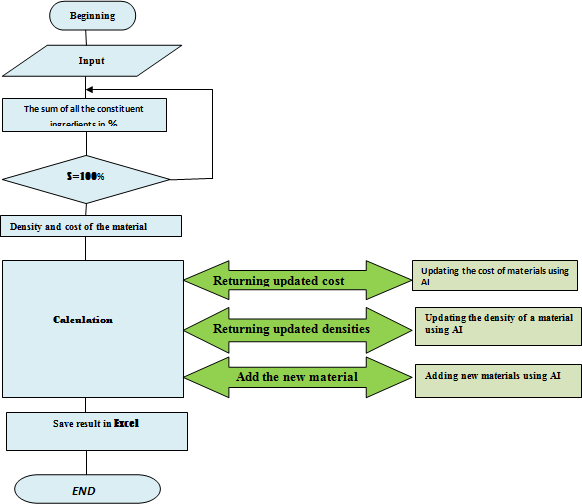
\includegraphics[width=0.65\textwidth]{media/ict3/image2}
	\caption*{Fig. 1 - The algorithm of the program code}
\end{figure}

\begin{multicols}{2}
This procedure allows us to graphically assess the effect of the
composition of man-made waste on the final cost of the construction mix
and, based on it, determine the optimal proportions.

But here it must be understood that any calculations must be supported
by laboratory experiments and field tests. The program code allows you
to automate the process of selecting the composition of a building mix
with additives from man-made raw materials, which in practice takes a
lot of time.

The user menu of the program code is developed using theTkinter library:

-The main library for creating a graphical user interface (GUI), which
allows you to build windows, input forms, buttons, tables, labels and
other interface elements.

{\bfseries Results and discussion.} For the development of the program
code, an algorithm was prepared, see Fig. 1, the principle of operation
of which is described below.

\emph{{\bfseries The algorithm works as follows:}}

Data for each ingredient of the construction mix with additives of
man-made raw materials is uploaded from the interface.

{\bfseries 1. Data initialization:}

The main() function sets the parameters for calculating the construction
mix:

-the volume of the mixture (volume) in m\textsuperscript{3};

-the density of the material (Material Densities) in kg /
m\textsuperscript{3};

-the percentage of the material (Material percentages);

-material costs (cost) per 1 kg.

\begin{enumerate}
\def\labelenumi{\arabic{enumi}.}
\setcounter{enumi}{1}
\item
  {\bfseries Mix Composition Calculation:}
\end{enumerate}

-the function calculate\_concrete\_mix(volume, densities, percentages,
costs) is called:

-a list to store mix composition data and a variable for the total cost
are initialized. For each ingredient;

The function returns:

-a list of data for the mix composition;

-the total cost of the mix.

Updating data on cost, density of materials, and adding new materials is
carried out using artificial intelligence.

{\bfseries 3. Saving Results to Excel:}

the function save\_to\_excel(data, file\_path) performs:

-creates an Excel file;

-adds table headers;

-writes rows containing mix composition data.

Formats the table:

-adjusts column widths;

-highlights headers with bold text and centers the text;

-sets the print area, page orientation, and scaling to fit the table to
one page width.

Saves the file to the specified path.

{\bfseries 4. Result Display:}

After saving the file, the program outputs:

-the path to the Excel file;

-the total cost of the construction mix.

{\bfseries 5. Program Execution:}

the program checks if it is the main module (if \_\_name\_\_ ==
"\_\_main\_\_":);

the main() function is called to perform the calculations and save the
results.

Fig. 2-11 show the program code of the program "Automated system for
selecting the composition of a building mix with additives from man-made
raw materials."
\end{multicols}

\begin{figure}[H]
	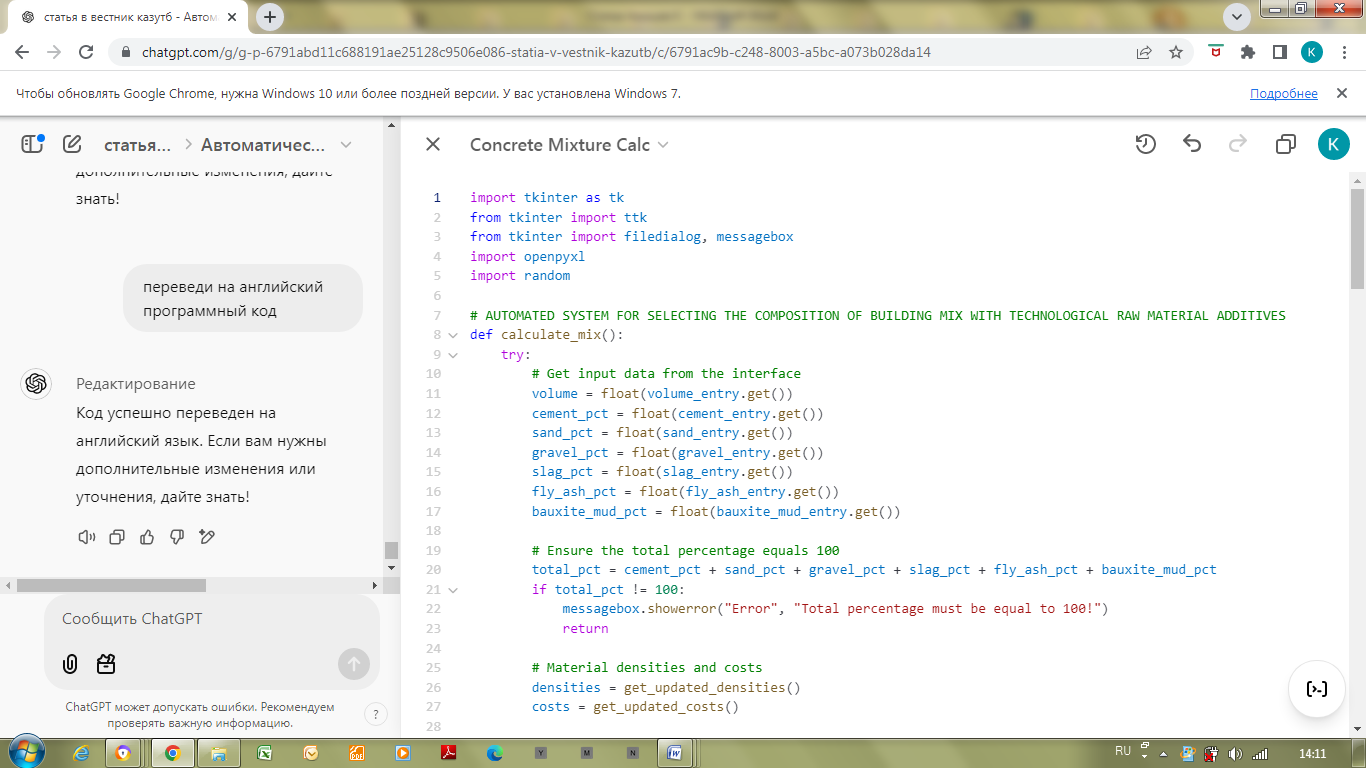
\includegraphics[width=0.8\textwidth]{media/ict3/image3}
	\caption*{Fig. 2 - Program code (Data entry)}
\end{figure}

\begin{figure}[H]
	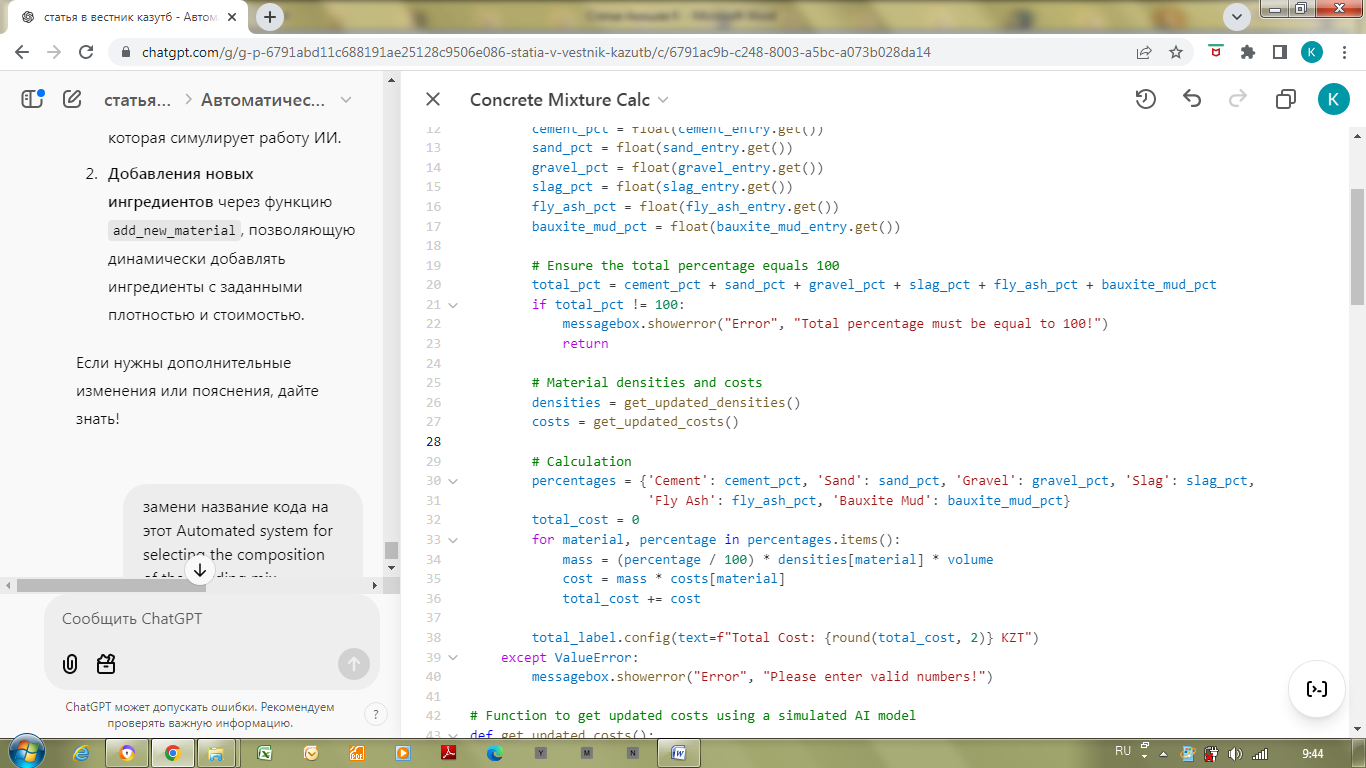
\includegraphics[width=0.7\textwidth]{media/ict3/image4}
	\caption*{Fig. 3 - Program code (Verification of compliance with the percentage of the building mix)}
\end{figure}

\begin{figure}[H]
	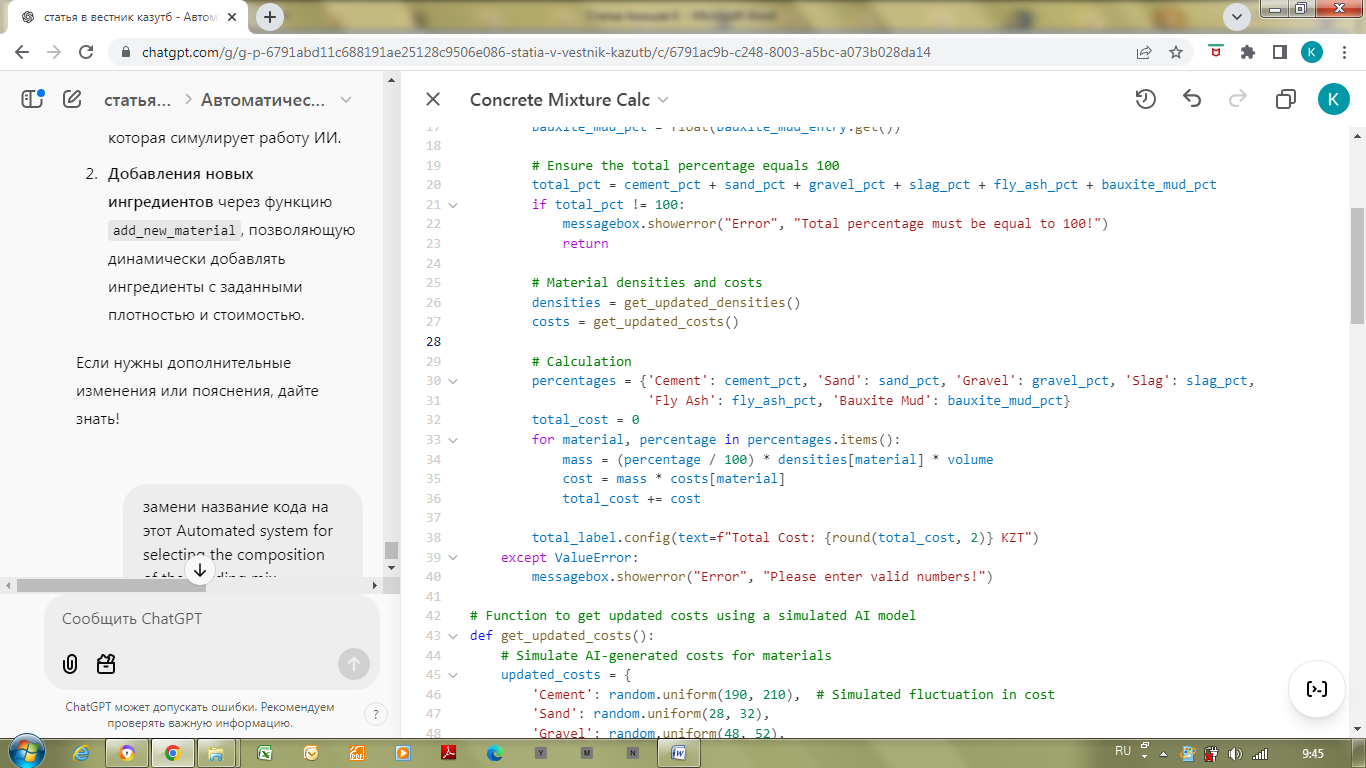
\includegraphics[width=0.35\textwidth]{media/ict3/image5}
	\caption*{Fig. 4 - Program code (Functions for determining the density and cost of the material)}
\end{figure}

\begin{figure}[H]
	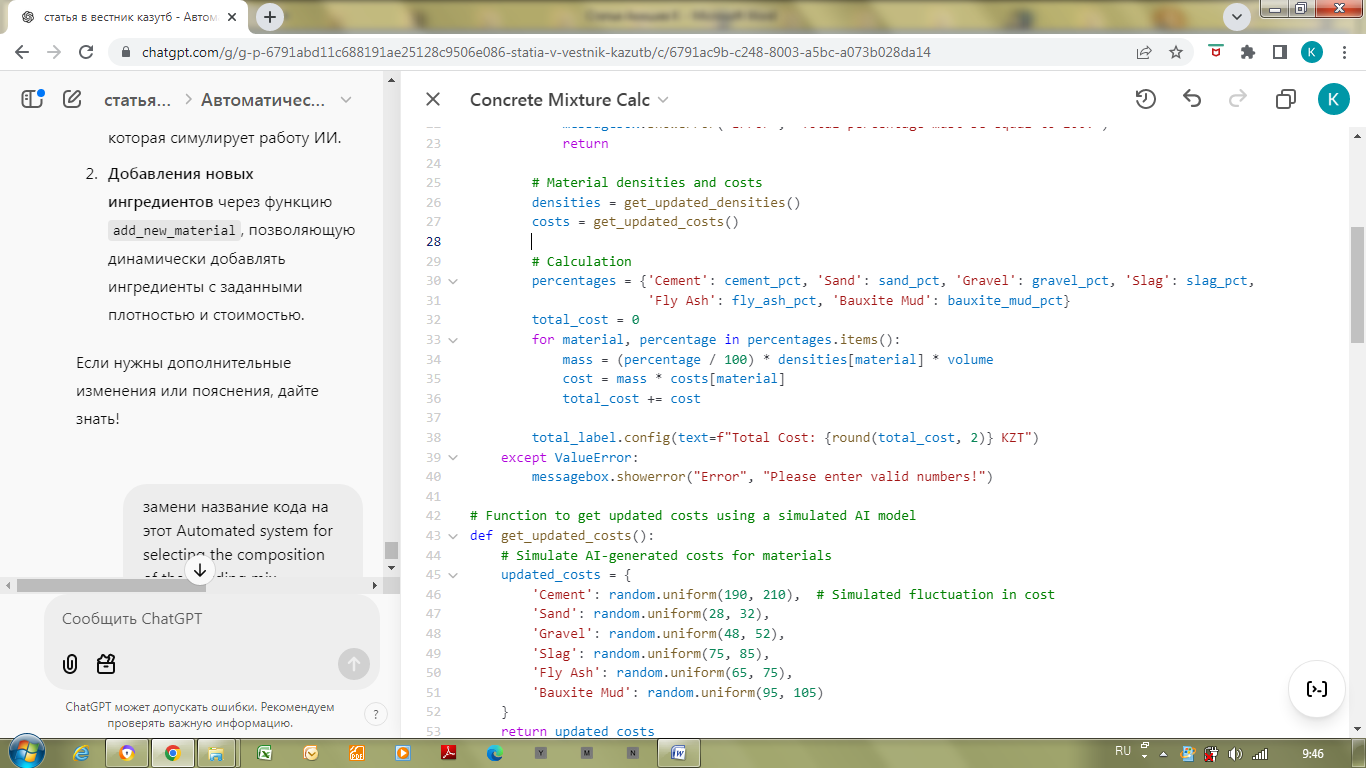
\includegraphics[width=0.8\textwidth]{media/ict3/image6}
	\caption*{Fig. 5 - Program code (Calculation)}
\end{figure}

\begin{figure}[H]
	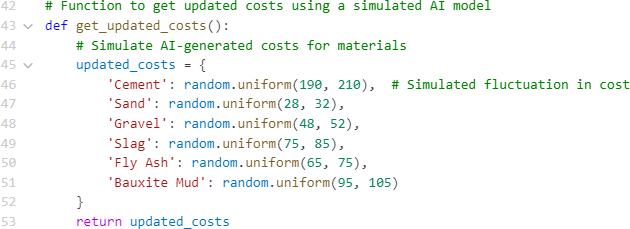
\includegraphics[width=0.55\textwidth]{media/ict3/image7}
	\caption*{Fig. 6 - Program code (Updating ingredients using AI)}
\end{figure}

\begin{figure}[H]
	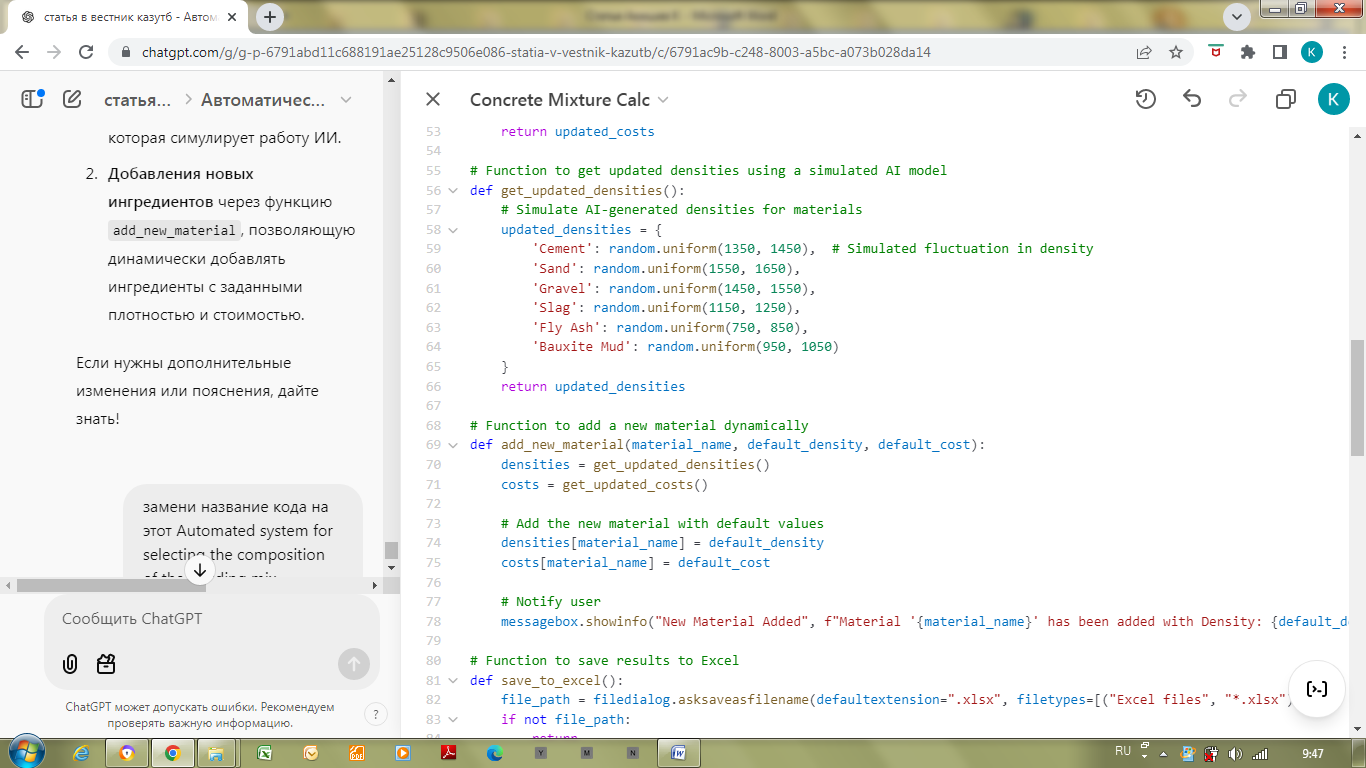
\includegraphics[width=0.6\textwidth]{media/ict3/image8}
	\caption*{Fig. 7 - Program code (Updating the density of the material using AI)}
\end{figure}

\begin{figure}[H]
	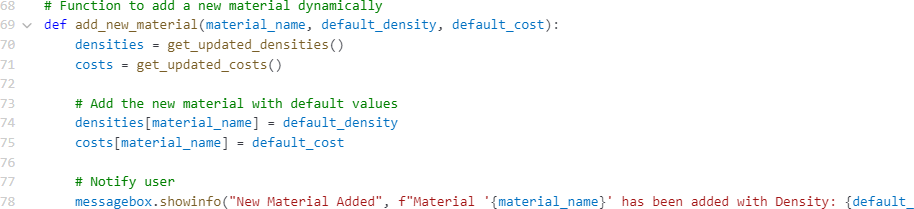
\includegraphics[width=0.8\textwidth]{media/ict3/image9}
	\caption*{Fig. 8 - Program code (Adding new materials)}
\end{figure}

\begin{figure}[H]
	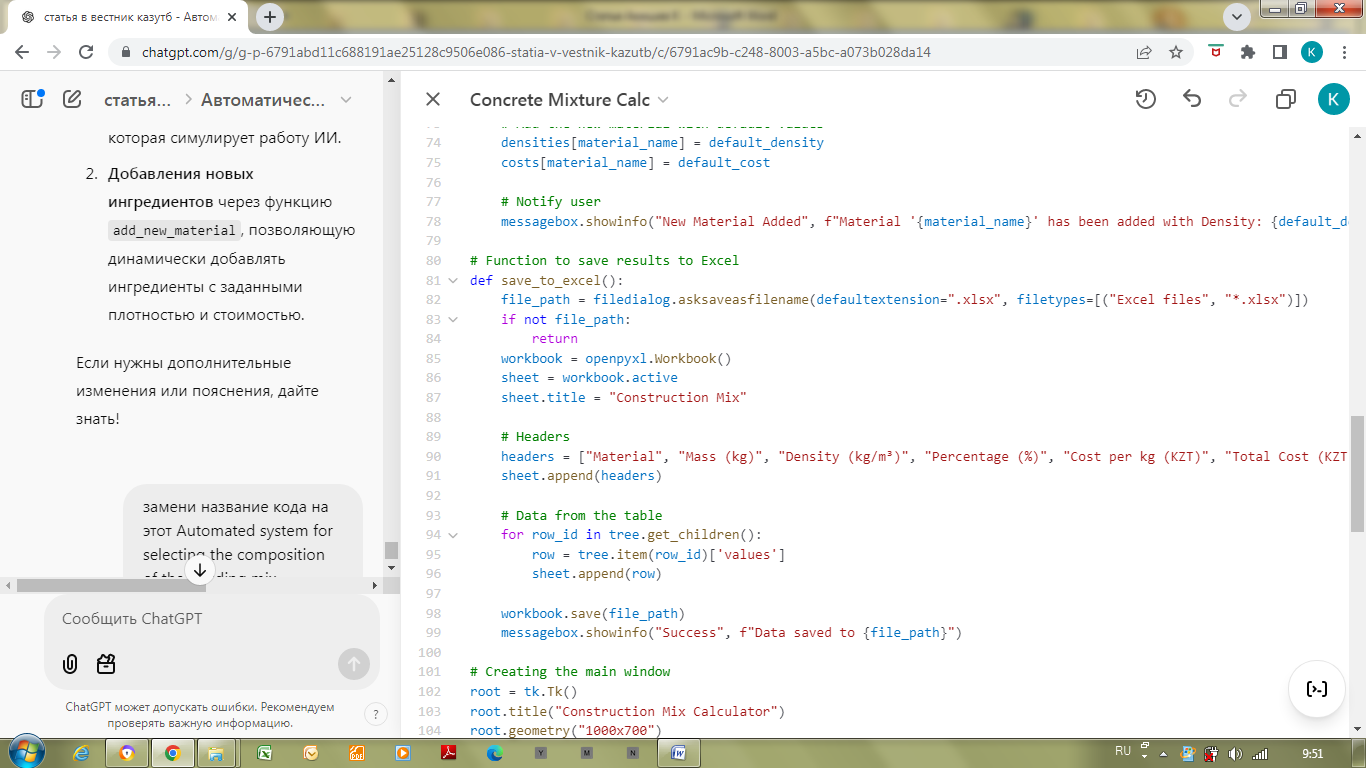
\includegraphics[width=0.8\textwidth]{media/ict3/image10}
	\caption*{Fig. 9 - Program code (Conversion of calculation results to Excel)}
\end{figure}

\begin{figure}[H]
	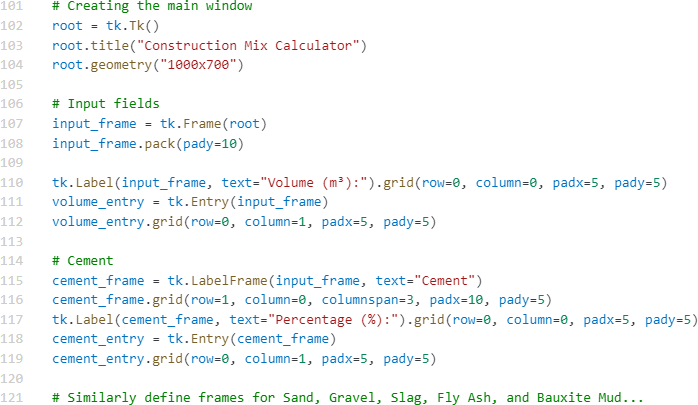
\includegraphics[width=0.6\textwidth]{media/ict3/image11}
	\caption*{Fig. 10 - Program code (Creating windows)}
\end{figure}

\begin{figure}[H]
	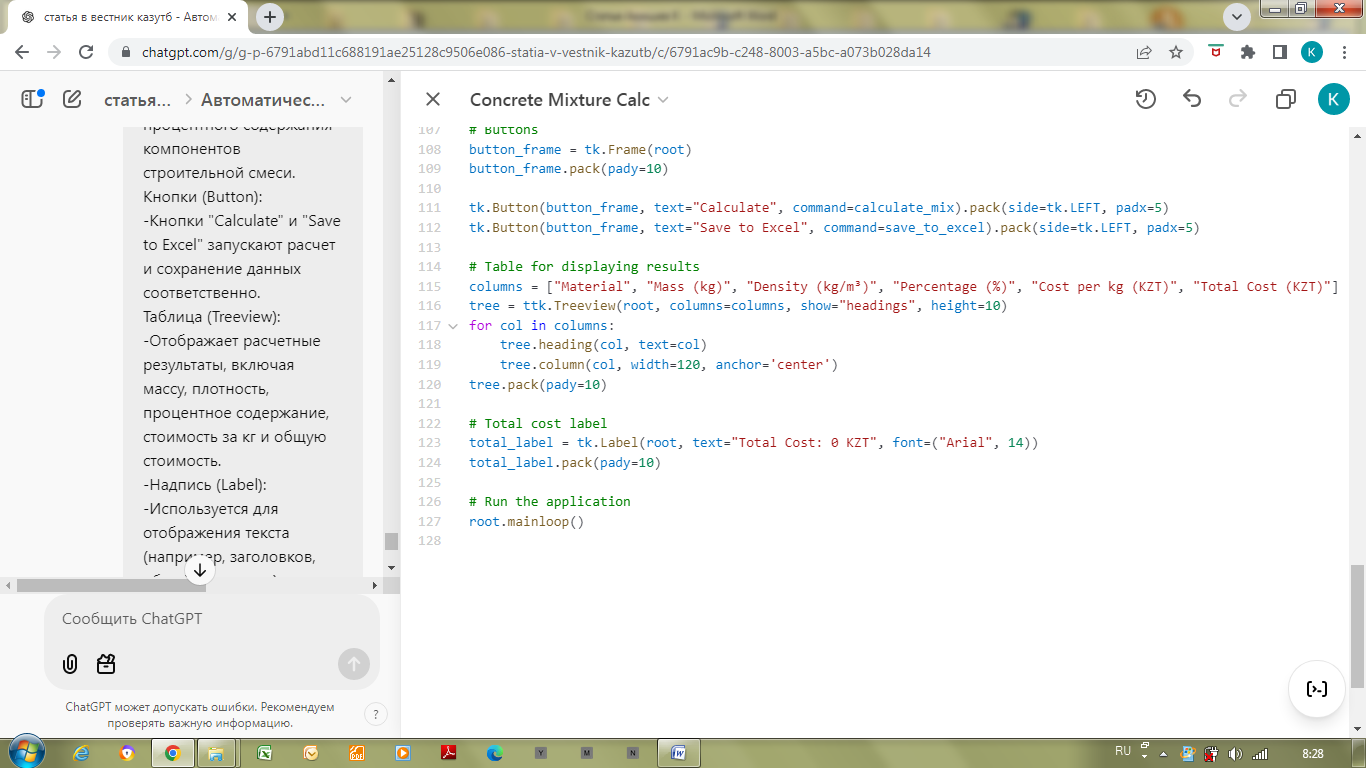
\includegraphics[width=0.2\textwidth]{media/ict3/image12}
	\caption*{Fig. 11 - Program code (program launch)}
\end{figure}

Figure 12 shows the menu interface of the program "Automated system for
selecting the composition of a building mix with additives from man-made
raw materials."

\begin{figure}[H]
	\centering
	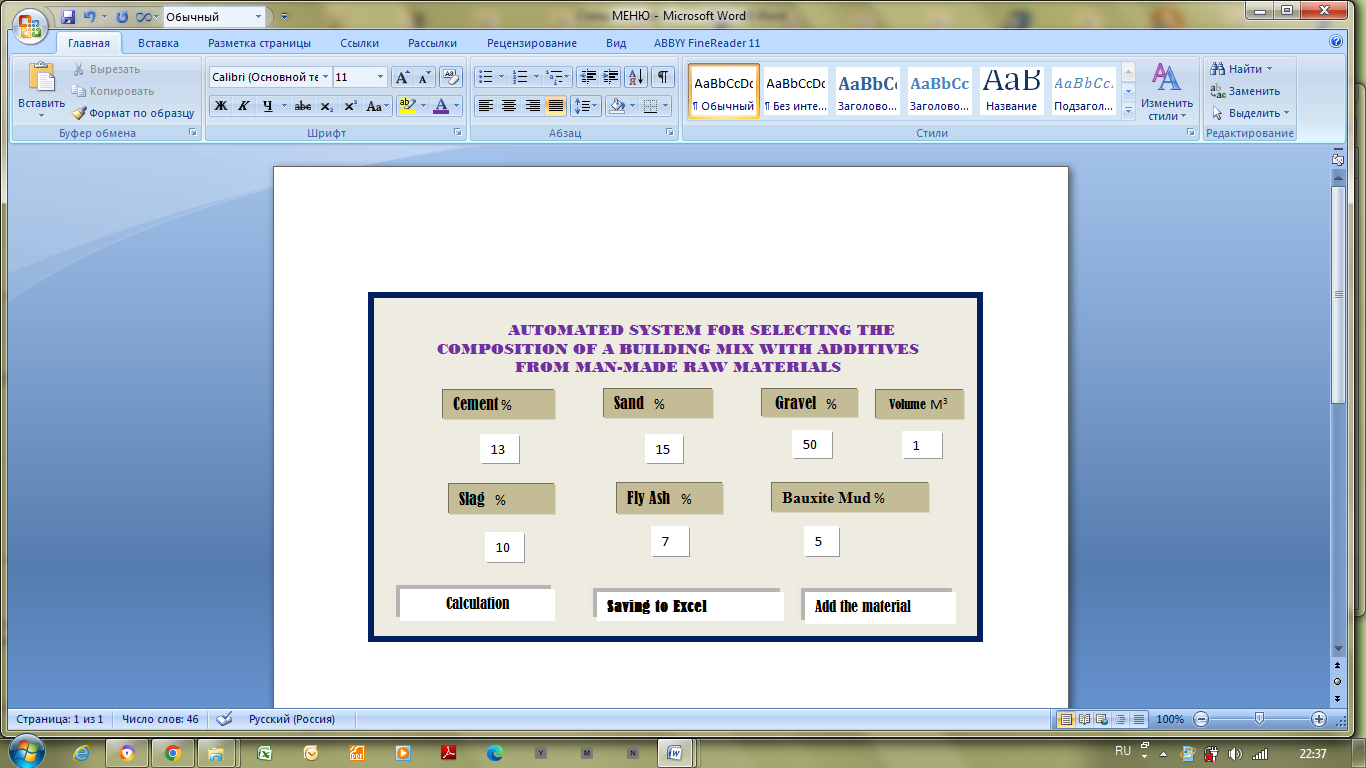
\includegraphics[width=0.8\textwidth]{media/ict3/image13}
	\caption*{Fig. 12 - Menu interface of the program "Automated system for selecting the composition of a building mix with additives from man-made raw materials"}
\end{figure}

\begin{table}[H]
\caption*{Table 1 - The results of calculating the selection of the building mix}
\centering
\begin{tblr}{ 
  colspec = {X[1] X[1] X[1] X[1] X[1] X[1]},
  cells = {c},
  hlines,
  vlines,
}
Material    & Percentage (\%) & Density (kg/m³) & Cost per kg (KZT) & Mass (kg) & Total Cost (KZT) \\
Cement      & 13              & 1400            & 200               & 182       & 36400            \\
Sand        & 15              & 1600            & 30                & 240       & 7200             \\
Gravel      & 50              & 1500            & 50                & 750       & 37500            \\
Slag        & 10              & 1200            & 80                & 120       & 9600             \\
Fly Ash     & 7               & 800             & 70                & 56        & 3920             \\
Bauxite Mud & 5               & 1000            & 100               & 50        & 5000             
\end{tblr}
\end{table}

\begin{multicols}{2}
User interaction with the program

1. Program launch:

the user launches the file. A window opens with fields for data entry.

2. Data entry:

The user enters:

the volume of the mixture (m3);

the percentage of each ingredient.

If necessary, you can add new ingredients.

3. Performing the calculation:

-clicking on the "Calculate" button starts the calculation.

Saving the results:

-the user clicks the "Save to Excel" button to save the results to a
file.

4. Adding new ingredients:

with the "Add Material" button, the user adds the ingredients that need
to be used in calculations.

Program operation:

The user enters:

Volume: 1 m3.

-cement: 13\%;

- sand: 15\%;

-Crushed stone: 50\%;

-slag: 10\%;

-fly ash: 7\%;

-Bauxite sludge: 5\%.

Presses the "Calculate" button. The program:

-verifies the correctness of the data;

-calculates the mass and cost of each ingredient.

-Determines the total cost of the construction mix depending on the
percentage composition.

Clicks "Save to Excel":

The program:

creates an Excel file and saves the data.

The results of calculating the selection of the building mix are
presented in Table 1.
\end{multicols}

If necessary, the user can add a new ingredient by clicking the "Add
Material" button. Table 2 shows the calculation results for the
percentage composition with other numerical values.

\begin{table}[H]
\caption*{Table 2 - Results of calculating the selection of the construction mixture}
\centering
\begin{tblr}{
  colspec = {X[1] X[1] X[1] X[1] X[1] X[1]},
  cells = {c},
  hlines,
  vlines,
}
Material    & Percentage (\%) & Density (kg/m³) & Cost per kg (KZT) & Mass (kg) & Total Cost (KZT) \\
Cement      & 14              & 1400            & 200               & 196       & 39200            \\
Sand        & 16              & 1600            & 30                & 256       & 7680             \\
Gravel      & 40              & 1500            & 50                & 600       & 30000            \\
Slag        & 15              & 1200            & 80                & 180       & 14400            \\
Fly Ash     & 10              & 800             & 70                & 80        & 5600             \\
Bauxite Mud & 5               & 1000            & 100               & 50        & 5000             
\end{tblr}
\end{table}

The program code has the ability to analyze data for different building
mix compositions. In particular, Fig. 13 shows a graph of the effect of
the percentage of man-made raw materials and building mixes on its cost.

\begin{figure}[H]
	\centering
	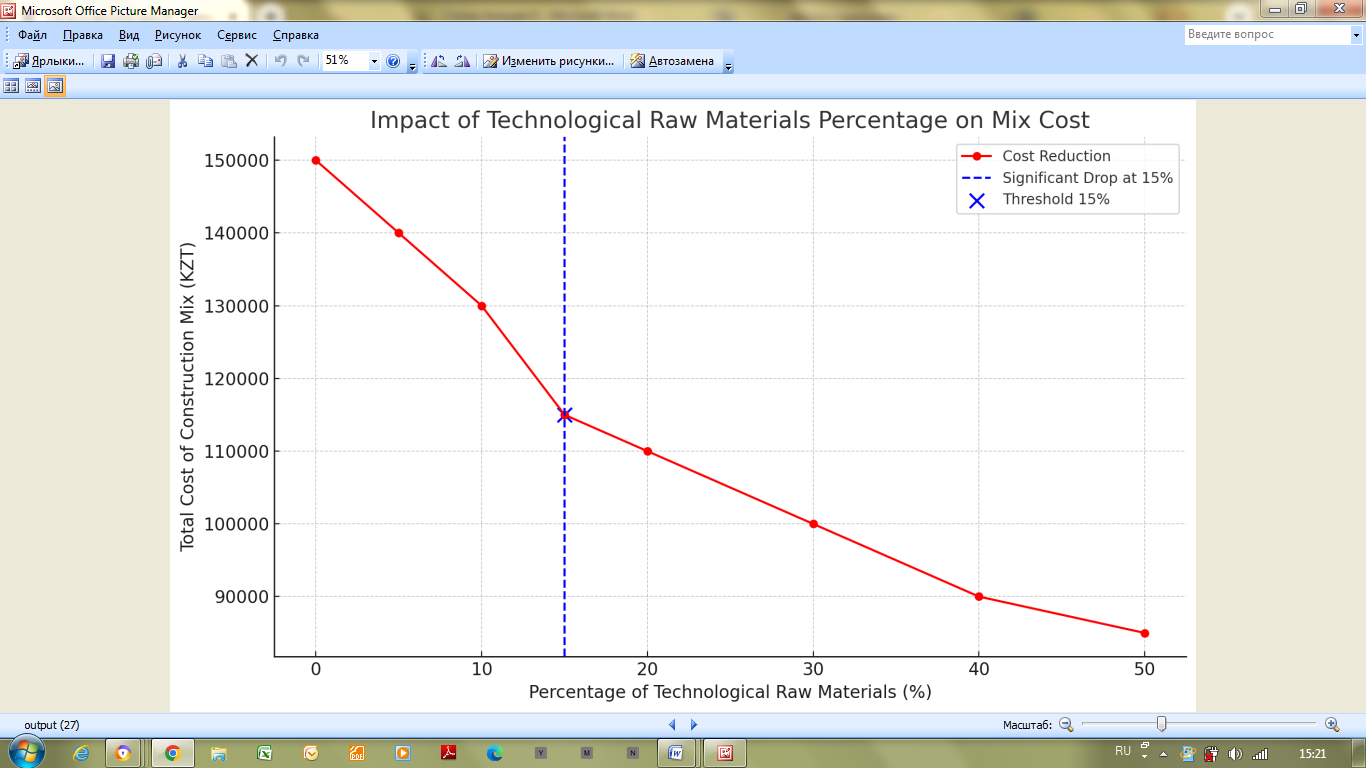
\includegraphics[width=0.8\textwidth]{media/ict3/image14}
	\caption*{Fig. 13 - Graph of the effect of the percentage composition of the building mix on its cost}
\end{figure}

\begin{multicols}{2}
As can be seen from the graph, when the composition of man-made raw
materials reaches 15\%, there is a significant reduction in the cost of
the construction mixture.

If necessary, various types of analysis can be obtained related to the
study of building mixes obtained as a result of automated selection.

{\bfseries Conclusion.} The proposed development methodology and the
developed program code are based on a flexible and modular approach that
allows automating the selection of building mixes using man-made raw
materials.

The scientific approach of the proposed methodology is based on:

- the use of mathematical modeling methods that ensure high accuracy of
calculations;

- realization of artificial intelligence capabilities for updating
information data;

-obtaining data analysis based on graphical representation of the
results of calculating the composition of the construction mixture with
additives of man-made raw materials.

The scientific novelty of the developed program consists in the
development of an original algorithm and the absence of analogues of the
source code, which allows obtaining both practical and scientific
results.

The developed program "Automated system for selecting the composition of
a building mix with additives from man-made raw materials" can be used
for practical purposes in business processes, small and medium-sized
businesses, during scientific experiments (master' s
degree, doctoral studies), in the educational process of the educational
program "Information Technology", Automation and Control, "Building
Materials".

The effectiveness of the developed program is incomparable with the
manual selection of a building mix and takes this process to a new
level.
\end{multicols}

\begin{center}
{\bfseries Referenses}
\end{center}

\begin{references}
1.Аkishev K. Inzhenernoe modelirovanie clozhnikh tekhnologicheskikh
sistem (proizvodstvo stroitelnikh izdelii s ispolzovanien tekhnogennikh
otkhodov. {[}Engineering modeling of complex technological systems
(production of construction products using man-made waste){]}. Lantar
books Publishing House, Almaty, 2023.-142s, 500 copies. ISBN
978-601-361-254-6 {[}in Russian{]}

2. Аkishev K and other{\bfseries .} Тhe use of simulation modeling in
calculating the productivity of the technological system for the
production of building products with fillers from man-made waste// NEWS
of the National Academy of Sciences of the Republic of Kazakhstan.-
Series of geology and technical sciences.-2024.-Vol. 4. (466)- P.
22--32. \href{https://doi.org/10.32014/2024.2518-170X.422}{DOI
10.32014/2024.2518-170X.422}

3. Аkishev K and other. Еvaluation of the efficiency of the
technological process for the production of building products with
fillers from metallurgical slag//Metalurgija.-2024.-63(2).- P. 267--27.

4. Аkishev K and other\emph{{\bfseries .}} Information technologies in the
management of technological processes for the production of building
products\emph{//} Eastern-European Journal of Enterprise
Technologies\emph{.-~}2024.- 1(2(127).-P. 66--73.
\href{https://doi.org/10.15587/1729-4061.2024.298480}{DOI
10.15587/1729-4061.2024.298480}

5. Chetan G. Kanapure and other. Interdisciplinary Approaches to AI,
Internet of Everything, and Machine Learning (2024).-рp.567-586).
-Artificial Intelligence in Automated Concrete Mix Design Using\\
Computerized Grading Curves{\bfseries .}
DOI\href{http://dx.doi.org/10.4018/979-8-3373-1032-9.ch036}{10.4018/979-8-3373-1032-9.ch036}

6. Vasileios Sergis, Claudiane M. Automating Mix Design for 3D Concrete
Printing Using Optimization Methods.- Digital
Discovery.-2022.-Vol.1(7).-P. 645-657.
\href{https://doi.org/10.1039/D2DD00040G}{DOI 10.1039/D2DD00040G}

7. Yaser Gamil and other. Frontier in Builit EnvironmentDigital
Transformation of Concrete Technology --A Review. -Sec/ Sustainable
Design and Constraction. -2022.-Vol.8
\href{https://doi.org/10.3389/fbuil.2022.835236}{DOI
10.3389/fbuil.2022.835236}

8.Jessica C. Forsdyke and other. Probabilistic Selection and Design of
Concrete Using Machine Learning// Data-Centric Engineering.-
2023.-Vol.4. DOI 10.1017/dce.2023.5

9. Atul Agrawal and other. From Concrete Mixture to Structural
Design A Holistic Optimization Procedure in the Presence of
Uncertainties.// Data-centric-engineering.-2023.e20.
\href{https://doi.org/10.1017/dce.2024.18}{DOI 10.1017/dce.2024.18}

10. Atul Agrawal and other. Data-centric-engineering.(2023) "From
Concrete Mixture to Structural Design A Holistic Optimization
Procedure in the Presence of Uncertainties" . Начало формы

11.Anna Corolina Rosa and other. Use of Operational Research Techniques
for Concrete Mix Design:A systematic review.// Heliyon.-
2023.-Vol.9(4):e15362
\href{https://doi.org/10.1016/j.heliyon.2023.e15362}{DOI
10.1016/j.heliyon.2023.e15362}

12. Haidong Tu and other. 16 (2023) . Recent advancements and future
trends in 3D concrete printing using waste materials// Developments in
the Built Environment.-2023.-Vol.16;100187\\
\href{https://doi.org/10.1016/j.dibe.2023.100187}{DOI
10.1016/j.dibe.2023.100187}

13. Egor Popello, Victoria GurievAutomation of the concrete mix
preparation process as a means to improve production efficiency//Matec
Web of Conferences.-2017.-Vol.129: 05003
DOI \\\href{http://dx.doi.org/10.1051/matecconf/201712905003}{10.1051/matecconf/201712905003}

13. S. Barbhuiya.Artificial Intelligence in Concrete Mix Design:
Advances, Applications, and Challenges, 2023 International Conference on
Innovation and Intelligence for Informatics, Computing, and Technologies
(3ICT). \href{http://dx.doi.org/10.1109/3ICT60104.2023.10391485}{DOI
10.1109/3ICT60104.2023.10391485}

14. Max Coenen and other. "Computer Vision as Key to an Automated
Concrete Production Control.2024.- P.26-33. Proceedings of the 41st
ISARC, Lille, France. ISBN 978-0-6458322-1-1, ISSN 2413-5844.
\href{https://doi.org/10.22260/ISARC2024/0005}{DOI
10.22260/ISARC2024/0005}

15. Santalova М.S., Soklakova I. V., Gorlov V.V., Muza U.А.
Avtomatizaciya proektnikh rabot v stroitelnoi kompanii v usloviyakh
cifrovizacii// Cifrivaya ekonomika.-2021.-Т.14.№2(53).-S.51-57. DOI\\
10.29030/2309-2076-2021-14-2-21-57. {[}in Russian{]}
\end{references}

\begin{authorinfo}
\emph{{\bfseries Information about the authors}}

Akishev K. M. - Candidate of Technical Sciences, Ass. Professor, Kazakh
University of Technology and Business named after K. Kulazhanov, Astana,
Kazakhstan, e -mail:akmail04cx@mail.ru;

Tulegulov A. D.- Candidate of physics and mathematics Sciences, Ass.
Professor, Kazakh University of Technology and Business named after. K.
Kulazhanov,Astana, Kazakhstan,e-mail:tud62@yandex.ru;

Nurtai Z.T. - Ph.D., Ass. Professor, Kazakh University of Technology and
Business named after. K. Kulazhanov,Astana, Kazakhstan, e-mail:
zhadira\_nurtai@mail.ru;

Akisheva L.- Nazarbayev Intellectual School, Astana, Republic of
Kazakhstan, e-mail: L. \href{mailto:Ak@mail.ru}{\nolinkurl{Ak@mail.ru}};

Biybosunov B.I.-Doctor of Physico-mathematical Sciences, Doctor of
Technical Sciences, Professor, Kyrgyz State University named after I.
Arabaev, Bishkek, Kyrgyzstan, e-mail: b.biibosunov@mail.ru;

Baizharikova M.M.-Candidate of Technical Sciences, Associate Professor,
Taraz Regional University, Taraz, Kazakhstan, e-mail:marina2288@mail.ru

\emph{{\bfseries Информация об авторах}}

Акишев К. М. -к.т.н., асс. профессор, Казахский университет технологии и
бизнеса им. К. Кулажанова, Астана, Казахстан, e-mail:akmail04cx@mail.ru;

Нуртай Ж.Т. - доктор PhD, асс. профессор, Казахский университет
технологии и бизнеса им. К. Кулажанова,

Астана, Казахстан, e-mail: zhadira\_nurtai@mail.ru

Акишева Л. -Назарбаев интеллектуальная школа, г. Астана, Казахстан,
e-mail: L.Ak@mail.ru;

Тулегулов А. Д.- к.ф.м.н., асс. профессор, Казахский университет
технологии и бизнеса им. К.Кулажанова, Астана, Казахстан:
e-mail:tud62@yandex.ru;

Бийбосынов Б.И.-д.ф.-м.н, д.т.н., профессор, Кыргызский Государственный
университет им. И. Арабаева, Бишкек, Кыргызстан,
e-mail:b.biibosunov@mail.ru;

Байжарикова М.М.-к.т.н., ассоциированный профессор, Таразский
Региональный университет, Тараз, Казахстан, e-mail: marina2288@mail.ru
\end{authorinfo}
